\addcontentsline{toc}{chapter}{Занятие 3. Процесс Пуассона}
\chapter*{Занятие 3. Процесс Пуассона}

\addcontentsline{toc}{section}{Контрольные вопросы и задания}
\section*{Контрольные вопросы и задания}

\subsubsection*{Приведите определение процесса Пуассона.}

$\left\{ N \left( t \right), \, t \geq 0 \right\} $ --- процесс Пуассона, если
\begin{enumerate}
  \item $N \left( 0 \right) = 0$;
  \item при $t_1 < t_2 < \dotsc < t_n$ события
  $$N \left( t_1 \right), N \left( t_2 \right) - N \left( t_1 \right), \dotsc,
    N \left( t_n \right) - N \left( t_{n - 1} \right) $$
  --- независимые;
  \item число событий на интервале зависит только от длины интервала,
  то есть есть однородность приращений
  $$N \left( t + s \right) - N \left( t \right) \overset{d}{=}
    N \left( s \right) \sim
    Pois \left( \lambda s \right).$$
\end{enumerate}

\subsubsection*{Запишите конечномерные распределения процесса Пуассона.}

Одномерные распределения
$$P \left\{ N \left( t \right) = k \right\} =
  e^{-\lambda t} \cdot \frac{ \left( \lambda t \right)^k}{k!}.$$

Двумерные распределения: $t_1 < t_2$.
Перейдём к приращениям
$$P \left\{ N \left( t_1 \right) = k_1, \, N \left( t_2 \right) = k_2 \right\} =
  P \left\{
    N \left( t_1 \right) = k_1, \, N \left( t_2 \right) - N \left( t_1 \right) = k_2 - k_1
  \right\} =$$
Случайная величина $N \left( t_1 \right) \sim Pois \left( \lambda t_1 \right) $, а
$N \left( t_2 \right) - N \left( t_1 \right) \sim
  Pois \left( \lambda \left( t_2 - t_1 \right) \right) $.
Совместная вероятность --- это произведение вероятностей
$$= e^{-\lambda t_1} \cdot \frac{ \left( \lambda t_1 \right)^{k_1}}{k_1!} \cdot
  e^{-\lambda \left( t_2 - t_1 \right) } \cdot
  \frac{ \left( \lambda \left( t_2 - t_1 \right) \right)^{k_2 - k_1}}{ \left( k_2 - k_1 \right)!}.$$

\subsubsection*{Какой вид имеют траектории процесса Пуассона?}

Траектория изображена на рисунке \ref{fig:3}.

\begin{figure}[h!]
  \centering
  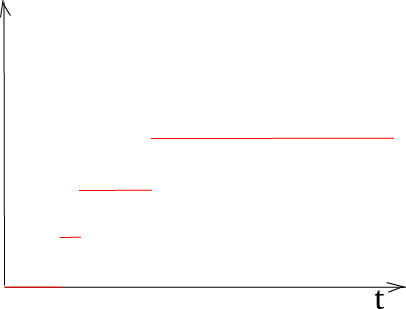
\includegraphics[width=.4\textwidth]{./pictures/3.png}
  \caption{График пуассоновского процесса}
  \label{fig:3}
\end{figure}

\subsubsection*{Какое содержание имеет параметр процесса Пуассона?}

$N \left( t \right) $ --- число событий, произошедших до момента времени $t$.

\addcontentsline{toc}{section}{Аудиторные задачи}
\section*{Аудиторные задачи}

\subsubsection*{3.2}

\textit{Задание.}
Пусть $ \left\{ N \left( t \right), \, t \geq 0 \right\} $ ---
процесс Пуассона с интенсивностью
$$ \lambda = 2.$$
Вычислите вероятности:
\begin{enumerate}[label=\alph*)]
  \item $P \left( N \left( 6 \right) = 3 \right) $;
  \item $P \left(
    N \left( 6 \right) = 3, \, N \left(9 \right) = 7, \, N \left( 15 \right) = 10 \right) $;
  \item $P \left( N \left( 6 \right) = 3 \; \middle| \; N \left( 9 \right) = 7 \right) $;
  \item $P \left( N \left( 9 \right) = 7 \; \middle| \; N \left( 6 \right) = 3 \right) $.
\end{enumerate}

\textit{Решение.}
\begin{enumerate}[label=\alph*)]
  \item $N \left( 6 \right) \sim Pois \left( 6 \cdot 2 \right) $, поэтому
  $$P \left( N \left( 6 \right) = 3 \right) =
    \frac{12^3}{3!} \cdot e^{-12};$$
  \item нужно перейти к приращениям, потому что они независимы
  \begin{gather*}
    P \left(
      N \left( 6 \right) = 3, \, N \left(9 \right) = 7, \, N \left( 15 \right) = 10 \right) = \\
    = P \left\{
      N \left( 6 \right) = 3, \, N \left( 9 \right) - N \left( 6 \right) = 4, \,
      N \left( 15 \right) - N \left( 9 \right) = 3 \right\} = \\
    = \left( \frac{12^3}{3!} \cdot e^{-12} \right) \cdot
    \left( \frac{6^4}{4!} \cdot e^{-6} \right) \cdot \left( \frac{12^3}{3!} \cdot e^{-12} \right);
  \end{gather*}
  \item по определению условной вероятности
  \begin{gather*}
    P \left( N \left( 6 \right) = 3 \; \middle| \; N \left( 9 \right) = 7 \right) =
    \frac{P \left( N \left( 6 \right) = 3, \, N \left( 9 \right) = 7 \right) }{P \left( N \left( 9 \right) = 7 \right) } = \\
    = \frac{ \frac{12^3}{3!} \cdot e^{-12} \cdot \frac{6^4}{4!} \cdot e^{-6}}{ \frac{18^7}{7!} \cdot e^{-18}} =
    \frac{12^3 \cdot 6^4 \cdot 7!}{3! \cdot 4! \cdot 18^7};
  \end{gather*}
  \item аналогично предыдущему пункту
  \begin{gather*}
    P \left( N \left( 9 \right) = 7 \; \middle| \; N \left( 6 \right) = 3 \right) =
    \frac{P \left( N \left( 9 \right) = 7, \, N \left( 6 \right) = 3 \right) }{P \left( N \left(6 \right) = 3 \right) } = \\
    = \frac{ \frac{12^3}{3!} \cdot e^{-12} \cdot \frac{6^4}{4!} \cdot e^{-6}}{ \frac{12^3}{3!} \cdot e^{-12}} =
    \frac{6^4}{4!} \cdot e^{-6} =
    \frac{P \left( N \left( 6 \right) = 3 \right) P \left( N \left( 3 \right) = 4 \right) }{P \left( N \left( 6 \right) = 3 \right) }.
  \end{gather*}
\end{enumerate}

\subsubsection*{3.3}

\textit{Задание.}
Пусть $ \left\{ N \left( t \right), \, t \geq 0 \right\} $ ---
процесс Пуассона с интенсивностью $ \lambda $.
Вычислите условное математическое ожидание
$M \left[ N \left( s \right) \; \middle| \; N \left( t \right) \right] $ для
$$0 \leq s \leq t.$$

\textit{Решение.}
Что ж такое условное математическое ожидание?

$N \left( s \right) $ и $N \left( t \right) $ --- дискретные величины, то есть
$$M \left[ N \left( s \right) \; \middle| \; N \left( t \right) \right] =
  \sum \limits_{l = 0}^{ \infty }
    l \cdot P \left\{ N \left( s \right) = l \; \middle| \; N \left( t \right) = k \right\}.$$
Отдельно посчитаем условную вероятность, а потом по ней возьмём математическое ожидание
$$P \left\{ N \left( s \right) = l \; \middle| \; N \left( t \right) = k \right\} =
  \frac{P \left\{ N \left( t \right) - N \left( s \right) = k - l \right\} P \left\{ N \left( s \right) = l \right\} }{P \left\{ N \left( t \right) = k \right\} } =$$
подставляем пуассоновские вероятности
$$= \frac{ \frac{ \left[ \lambda \left( t - s \right) \right]^{k - l}}{ \left( k - l \right)!} \cdot e^{-\lambda \left( t - s \right) }}{ \frac{ \left( \lambda t \right)^k}{k!} \cdot e^{-\lambda t}} \cdot
  \frac{ \left( \lambda s \right)^l}{l!} \cdot e^{-\lambda l} =
  \frac{k! \left( t - s \right)^{k - l} s^l}{ \left( k - l \right)! l! t^k} =
  C_k^l \cdot \left( \frac{t - s}{t} \right)^{k - l} \cdot \left( \frac{s}{t} \right)^l.$$
Имеем биномиальное распределение с параметрами $k$ и $ \frac{s}{t}$.

Вывод: при условии $N \left( t \right) = k$ мы нашли распределение
$$N \left( s \right) \sim
  B \left( k, \frac{s}{t} \right).$$

Условное математическое ожидание
$$M \left[ N \left( s \right) \; \middle| N \left( t \right) = k \right] =
  \frac{ks}{t}.$$

Ответ: $ \frac{N \left( t \right) \cdot s}{t}$.
Куда пропала сумма?

$$M \left[ N \left( s \right) \; \middle| \; N \left( t \right) = k \right] =
  \sum \limits_l
    l \cdot P \left[ N \left( s \right) = l \; \middle| \; N \left( t \right) = k \right] =$$
Нашли эту вероятность
$$= \sum \limits_l l \cdot P \left\{ Bin \left( k, \frac{s}{t} \right) = l \right\} =
MBin \left( k, \frac{s}{t} \right) =
k \cdot \frac{s}{t}.$$

Условное математическое ожидание --- это математическое ожидание по условному распределению.

\subsubsection*{3.4}

\textit{Задание.}
Пусть $N = \left\{ N \left( t \right), \, t \geq 0 \right\} $ ---
процесс Пуассона с интенсивностью $ \lambda $.
Найдите вероятность того, что первый прыжок процесса $N$ произошёл до момента времени
$s \in \left[ 0, t \right] $ при условии,
что на отрезке $ \left[ 0, t \right] $ произошло ровно $n$ прыжков.

\textit{Решение.}
Нужно найти вероятность $P$(первый прыжок произошёл до момента
$\left. s \in \left[ 0, t \right] \right| N \left( t \right) = n$).
Нужно это условие переписать через пуассоновский процесс.
Получаем
$P$(первый прыжок произошёл до момента
  $\left. s \in \left[ 0, t \right] \right| N \left( t \right) = n$) =
  $P \left\{ N \left( s \right) \geq 1 \; \middle| \; N \left( t \right) = n \right\} $.
Значения зависимые
$$P \left\{ N \left( s \right) \geq 1 \; \middle| \; N \left( t \right) = n \right\} =
  1 - P \left\{ N \left( s \right) = 0 \; \middle| \; N \left( t \right) = n \right\} =$$
Условное распределение биномиальное
\begin{gather*}
  = 1 - P \left\{ Bin \left( n, \frac{s}{t} \right) = 0 \right\} =
  1 - C_n^0 \cdot \left( \frac{s}{t} \right)^0 \cdot \left( 1 - \frac{s}{t} \right)^{n - 0} =
  1 - \left( 1 - \frac{s}{t} \right)^n.
\end{gather*}

\subsubsection*{3.5}

\textit{Задание.}
Пусть $N = \left\{ N \left( t \right), \, t \geq 0 \right\} $
является процессом Пуассона с параметром $ \lambda $.
Докажите, что при условии, что $N$ имеет ровно 1 прыжок на отрезке $ \left[ a, b \right] $,
момент этого прыжка является равномерно распределённой на отрезке $ \left[ a, b \right] $
случайной величиной.

\textit{Решение.}
Обозначим $ \tau $ --- момент прыжка на отрезке $ \left[ a, b \right] $.
Нужно найти
$P \left\{ \tau \leq t \; \middle| \; N \left( b \right) - N \left( a \right) = 1 \right\} =
  P \left\{
    N \left( t \right) - N \left( a \right) = 1 \; \middle| \;
    N \left( b \right) - N \left( a \right) = 1 \right\} $.

Изобразим процесс на графике \ref{fig:35}.

\begin{figure}[h!]
  \centering
  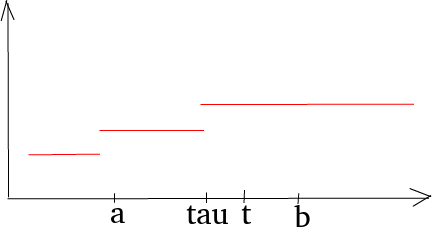
\includegraphics[width=.4\textwidth]{./pictures/3_5.png}
  \caption{График пуассоновского процесса}
  \label{fig:35}
\end{figure}

У пуассоновского процесса есть однородность приращений
\begin{gather*}
  P \left\{
    N \left( t \right) - N \left( a \right) = 1 \; \middle| \;
    N \left( b \right) - N \left( a \right) = 1 \right\} =
  P \left\{ N \left( t - a \right) = 1 \; \middle| \; N \left( b - a \right) = 1 \right\} = \\
  = P \left\{ Bin \left( 1, \frac{t - a}{b - a} \right) = 1 \right\} =
\end{gather*}
Это бернуллиевская величина
$$= \frac{t - a}{b - a}.$$
Получилось равномерное распределение, что и требовалось доказать.

\subsubsection*{3.6}

\textit{Задание.}
Пусть $ \left\{ \tau_k \right\}_{k \geq 1}$ --- последовательность независимых показательно
распределённых случаных величин с параметром $ \lambda $.
Положим
$$T_0 = 0, \,
  T_n = \sum \limits_{k = 1}^n \tau_k, \,
  n \geq 1; \,
  \nu \left( t \right) = \max \left( n \, : \, T_n \leq t \right), \,
  t \geq 0.$$
\begin{enumerate}[label=\alph*)]
  \item Докажите, что
  $$ \lim \limits_{n \to \infty } \frac{T_n}{n} =
    \frac{1}{ \lambda }$$
  почти наверное.
  \item Докажите, что случайная величина $ \tau_1 = T_{ \nu \left( t \right) + 1} - t$
  имеет показательное распределение с параметром $ \lambda $.
  \item Докажите, что $ \left\{ \nu \left( t \right), \, t \geq 0 \right\} $
  является процессом Пуассона с интенсивностью $ \lambda $.
\end{enumerate}

\textit{Решение.}
$\nu \left( t \right) = \max \left( n \, : \, T_n \leq t \right) $ --- случайный процесс.

Посмотрим, как этот процесс выглядит (рис. \ref{fig:36}).

$T_n$ --- это накопительные суммы.

В момент $T_1$ только $T_1 \leq t$, то есть от $T_1$ до $T_2$ значение процесса будет равно единице.

\begin{figure}[h!]
  \centering
  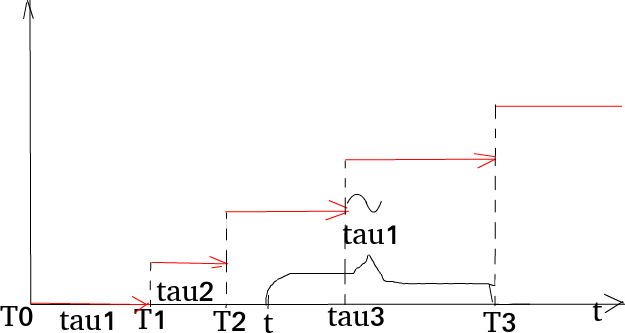
\includegraphics[width=.4\textwidth]{./pictures/3_6.png}
  \caption{График процесса}
  \label{fig:36}
\end{figure}

Тут расставили стрелочки, то ест $ \nu $ --- это непрерывная справа функция.
То есть $ \nu $ --- это модификация пуассоновского процесса.
Конечномерные распределения несут ещё не всю информацию.

\begin{enumerate}[label=\alph*)]
  \item Нужно доказать, что
  $$ \lim \limits_{n \to \infty } \frac{T_n}{n} =
    \frac{1}{ \lambda }$$
  почти наверное.

  Это равенство --- это просто закон больших чисел, потому что
  $$ \frac{1}{n} \sum \limits_{k = 1}^n \tau_k = T_n \to
    M \tau_1 = \frac{1}{ \lambda }.$$

  Сумма $T_n$ сходится к бесконечности.
  Это нужно для того, чтобы определить процесс на всей оси.
  То есть вывод из пункта a) следующий
  $$T_n =
    n \cdot \frac{T_n}{n} \to
    \infty \cdot \frac{1}{ \lambda } =
    \infty $$
  и $ \nu \left( t \right) $ определено при всех $t$.
  \item $ \tilde{ \tau_1}$ --- это величина до следующего прыжка.

  Этот пункт означает, что процесс $ \nu $ имеет однородные приращения.

  Докажем, чо $ \tilde{ \tau_1}$ имеет действительно показательное распределение.
  Проще всего для показательного распределения посчитать
  $$P \left( \tilde{ \tau_1} \right) =
    1 - F =
    1 - \left( 1 - e^{-\lambda s} \right) =
    e^{-\lambda s},$$
  где $F$ --- функция распределения.
  Вопрос: есть ли такое равенство.

  Значит,
  $P \left( \tilde{ \tau_1} > s \right) =
    P \left( T_{ \nu \left( t \right) + 1} > t + s \right) $.
  Величина $T$ берётся в случайный момент.
  Такая вероятность может быть записана через сумму по всем возможным $T$, то есть
  $$P \left( T_{ \nu \left( t \right) + 1} > t + s \right) =
    \sum \limits_{n = 0}^{ \infty }
      P \left( T_n \leq t < T_{n + 1}, \, T_{n + 1} > t + s \right) =$$
  Одно условие убирается
  $$ = \sum \limits_{k = 0}^{ \infty } P \left( T_n \leq t, T_{n + 1} \leq t + s \right) =$$
  Момент $T_{n + 1}$ --- это момент следующего скачка после $T_n$.
  Тогда
  \begin{gather*}
    = \sum \limits_{n = 0}^{ \infty }
      P \left( T_n \leq t, \, T_n + \tau_{n + 1} > t + s \right) = \\
    = \sum \limits_{n = 0}^{ \infty }
      P \left\{ T_n \leq t, \tau_{n + 1} \geq \left( t - T_n \right) + s \right\} =
  \end{gather*}
  Моменты $ \tau_{n + 1}$ и $T_n$ --- независимые величины.
  $$= \sum \limits_{n = 0}^{ \infty }
    MP \left[ T_n \leq t, \, \tau_{n + 1} > \left( t - T_n \right) + s \; \middle| \;
    T_n \right] =$$
  Вспомним, какая вероятность $P \left( \tau > x \right) = e^{-\lambda x}$.
  Тогда
  $$P \left( \tau > x + y \right) =
    e^{-\lambda \left( x + y \right) } =
    e^{-\lambda x} e^{-\lambda y}.$$
  Для показательных величин выполнено соотношение
  $$P \left( \tau > x + y \right) =
    e^{-\lambda y} P \left( \tau > x \right) $$
  --- свойство отсутствия последействия.
  $$= \sum \limits_{n = 0}^{ \infty }
      e^{-\lambda s} P \left( T_n \leq t, \tau_{n + 1} > t - T_n \right) =
    e^{-\lambda s} \sum \limits_{n = 0}^{ \infty } P \left( T_n \leq t < T_{n + 1} \right) =$$
  Такая сумма равна единице,
  потому что $t$ всегда попадает между $T_n$ и $T_{n + 1}$ при каком-то $n$, потому
  $$= e^{-\lambda s},$$
  так что такая величина $ \tilde{ \tau_1}$ действительно имеет показательное распределение.
  \item Найдём конечномерные распределения $ \nu \left( t \right) $.
  Имеем
  \begin{gather*}
    P \left\{
      \nu \left( t_1 \right) = k_1, \nu \left( t_2 \right) = k_2, \dotsc,
      \nu \left( t_n \right) = k_n
    \right\} = \\
    = P \left(
      \sum \limits_{l = 1}^{k_1} \tau_l \leq t_1 < \sum \limits_{l = 1}^{k_1 + 1} \tau_l, \dotsc,
      \sum \limits_{l = 1}^{k_n} \tau_l \leq t_n < \sum \limits_{l = 1}^{k_n + 1} \tau_l
    \right) = \\
    = \idotsint \limits_{k_n + 1}
      \lambda^{k_n + 1} e^{-\lambda \left( x_{k_1} + \dotsc + x_{k_n} + 1 \right) }
    dx_{k_n + 1} \dotsc dx_1 = \\
    = \lambda^{k_n + 1} \cdot
    \idotsint \limits_{k_n, \, 0 < x_{k_1} + \dotsc + x_{k_n} \leq t, \, t = \sum t_i}
      e^{-\lambda \left( x_{k_1} + \dotsc + x_{k_n} \right) } \times \\
       \times \int \limits_{t - \sum \limits_{i = 1}^{k_n} x_i}
        e^{-\lambda x_{k_n + 1}} dx_{k_n + 1} \dotsc dx_1 =
  \end{gather*}
  Возьмём последний интеграл
  $$ \int \limits_{t - \sum \limits_{i = 1}^{k_n} x_i} e^{-\lambda x_{k_n + 1}} dx_{k_n + 1} =
    \left.
      -\frac{1}{ \lambda } \cdot e^{-\lambda x_{k_n + 1}}
    \right|_{t - \sum \limits_{i = 1}^{k_n} x_i}^{+ \infty }.$$
  Подставляем и получаем
  \begin{gather*}
    = \frac{ \lambda^{k_n + 1}}{ \lambda }
    \idotsint \limits_{k_n, \, 0 < x_{k_1} + \dotsc + x_{k_n} \leq t}
      e^{-\lambda \sum \limits_{i = k_1}^{k_n} x_i}
      e^{-\lambda t + \lambda \sum \limits_{i = k_1}^{k_n} x_i} dx_{k_n} \dotsc dx_{k_1} = \\
   = \lambda^{k_n} e^{-\lambda t}
   \idotsint \limits_{0 < \sum \limits_{i = k_1}^{k_n} x_i \leq 1} dx_{k_n} \dotsc dx_{k_1} =
 \end{gather*}
  Чтобы понять, чему будет равен этот интеграл, рассмотрим частные случаи:
  \begin{enumerate}
    \item когда есть двойной интеграл
    \begin{gather*}
      \iint \limits_{0 < x_1 + x_2 \leq t} dx_2 dx_1 =
      \int \limits_0^t \int \limits_0^{t - x_1} dx_2 dx_1 =
      \int \limits_0^t \left. x_2 \right|_0^{t - x_1} dx_1 = \\
       =\int \limits_0^t \left( t - x_1 \right) dx_1 =
      t \int \limits_0^t dx_1 - \int \limits_0^t x_1 dx_1 =
      t^2 - \left. \frac{x^2}{2} \right|_0^t =
      t^2 - \frac{t^2}{2} = \\
      = \frac{t^2}{2} =
      \frac{t^2}{2!};
    \end{gather*}
    \item когда есть тройной интеграл
    \begin{gather*}\iiint \limits_{0 < x_1 + x_2 + x_3 \leq t} dx_3 dx_2 dx_1 =
      \int \limits_0^t \int \limits_0^{t - x_1} \int \limits_0^{t - x_1 - x_2} dx_3 dx_2 dx_1 = \\
      = \int \limits_0^t \int \limits_0^{t - x_1} \left( t - x_1 - x_2 \right) dx_2 dx_1 = \\
      = \int \limits_0^t \left(
        t \int \limits_0^{t - x_1} dx_2 - x_1 \int \limits_0^{t - x_1} dx_2 -
        \int \limits_0^{t - x_1} x_2 dx_2 \right) dx_1 = \\
      = \int \limits_0^t \left[
        t \left( t - x_1 \right) - x_1 \left( t - x_1 \right) - \frac{ \left( t - x_1 \right)^2}{2}
      \right] dx_1 = \\
      = \int \limits_0^t
        \frac{2t^2 - 2tx_1 - 2tx_1 + 2x_1^2 - t^2 + 2tx_1 - x_1^2}{2} dx_1 \times \\
      \times \int \limits_0^t \frac{t^2 - 2x_1 t + x_1^2}{2} dx_1 =
      \int \limits_0^t \frac{ \left( t - x_1 \right)^2}{2} dx_1 =
      \left. -\frac{1}{2} \cdot \frac{ \left( t - x_1 \right)^3}{3} \right|_0^t = \\
      = \frac{t^3}{2 \cdot 3} =
      \frac{t^3}{3!}.
    \end{gather*}
  \end{enumerate}
  Значит,
  $$ \idotsint \limits_{0 < \sum \limits_{i = k_1}^{k_n} x_i \leq 1} dx_{k_n} \dotsc dx_{k_1} =
    \frac{t^{k_n}}{k_n!}.$$

  Тогда вероятность равна
  $$= \frac{ \lambda^{k_n} e^{-\lambda t} t^{k_n}}{k_n!} =
    \frac{ \left( \lambda t \right)^{k_n}}{k_n!} \cdot e^{-\lambda t}.$$
  Получился процесс Пуассона с интенсивностью $ \lambda $.
\end{enumerate}

\subsubsection*{3.7}

\textit{Задание.}
Пусть $N = \left\{ N \left( t \right), \, t \geq 0 \right\} $ ---
процесс Пуассона с параметром $ \lambda $ и пусть $ \left\{ Y_n \right\}_{n \geq 1}$ ---
независимая от $N$ последовательность независимых бернуллиевских случайных величин с парметром
$p \in \left( 0, 1 \right) $.
Положим
$$S_n = Y_1 + \dotsc + Y_n.$$
Докажите, что процесс $ \xi = \left\{ S_{N \left( t \right)}, \, t \geq 0 \right\} $
является процессом Пуассона с параметром $ \lambda t$.

\textit{Решение.}
Пуассоновский процесс
$$N \left( t \right) =
  \sum \limits_{n = 1}^{N \left( t \right) } 1$$
--- число событий до момента $N \left( t \right) $.
В $ \xi $ складываем не 1, а $Y_i = 0$ или $1$.

Начнём с того, что посчитаем одномерные распределения и посмотрим,
что это тоже пуассоновские величины.
Есть сумма случайного числа слагаемых.
Нужно перебирать все возможные значения $N \left( t \right) $.
Имеем
\begin{gather*}
  P \left\{ S_{N \left( t \right) } = k \right\} =
  P \left\{ Y_1 + \dotsc + Y_{N \left( t \right) } = k \right\} = \\
  = \sum \limits_{n = 0}^{ \infty }
    P \left\{ N \left( t \right) = n, \, Y_1 + \dotsc + Y_n = k \right\} =
\end{gather*}
Сумма $Y_1 + \dotsc + Y_n $ --- биномиальная величина
$$= \sum \limits_{n = k}^{ \infty }
    \frac{ \left( \lambda t \right)^n}{n!} \cdot
    e^{-\lambda t} \cdot C_n^k p^k \left( 1 - p \right)^{n - k} =$$
Преобразуем
$$= e^{-\lambda t} p^k \cdot
  \sum \limits_{n = k}^{ \infty }
    \frac{ \left( \lambda t \right)^n}{n!} \cdot C_n^k \left( 1 - p \right)^{n - k} =$$
Распишем $C_n^k$ явно
$$= e^{-\lambda t} p^k \cdot
  \sum \limits_{n = k}^{ \infty }
    \frac{ \left( \lambda t \right)^n}{n!} \cdot
    \frac{n!}{k! \left( n - k \right)!} \cdot \left( 1 - p \right)^{n - k} =
  \frac{e^{-\lambda t} p^k}{k!} \cdot
  \sum \limits_{n = k}^{ \infty }
    \frac{ \left( \lambda t \right)^{n + k} \left( 1 - p \right)^{n - k}}{ \left( n - k \right)!} =$$
Имеем ряд для экспоненты.
Заменим $n - k$ на новый индекс суммирования
$$= \frac{e^{-\lambda t} p^k}{k!} \cdot
  \sum \limits_{n = 0}^{ \infty }
    \frac{ \left( \lambda t \right)^{n + k} \left( 1-  p \right)^n}{n!} =$$
Выносим $ \left( \lambda t \right)^k$ за знак суммы
$$= \frac{e^{-\lambda t} p^k \left( \lambda t \right)^k}{k!} \cdot
  \sum \limits_{n = 0}^{ \infty } \frac{ \left( \lambda t \right)^n \left( 1 - p \right)^n}{n!} =
  \frac{e^{-\lambda t} \left(p \lambda t \right)^k}{k!} \cdot e^{ \lambda t \left( 1 - p \right) } =
  \frac{e^{-\lambda pt} \left( \lambda pt \right)^k}{k!}$$
--- пуассоновская вероятность.

Вывод: $S_{N \left( t \right) } \sim Pois \left( \lambda pt \right) $,
то есть у такого процесса одномерные распределения такие же,
как у пуассоновского с параметром $ \lambda pt$.

\addcontentsline{toc}{section}{Домашнее задание}
\section*{Домашнее задание}

\subsubsection*{3.11}

\textit{Задание.}
Пусть $N = \left\{ N \left( t \right), \, t \geq 0 \right\} $ ---
процесс Пуассона с интенсивностью $ \lambda = 5$.
Вычислите вероятности:
\begin{enumerate}[label=\alph*)]
  \item $P \left( N \left( 2 \right) \geq 3, \, N \left( 5 \right) \leq 4 \right) $;
  \item $P \left(
    N \left( 2 \right) \geq 3, \, N \left( 3 \right) \geq 4, \, N \left( 5 \right) \leq 3 \right) $;
  \item $P \left(
    N \left( 2 \right) = 3, \, N \left( 3 \right) = 5, \, N \left( 4 \right) \leq 6 \right) $;
  \item $P \left( N \left( 2 \right) = 3 \; \middle| \; N \left( 3 \right) = 5 \right) $;
  \item $P \left( N \left( 3 \right) = 5 \; \middle| \; N \left( 2 \right) = 3 \right) $.
\end{enumerate}

\textit{Решение.}
\begin{enumerate}[label=\alph*)]
  \item Рассмотрим все возможные случаи
  \begin{gather*}
    P \left( N \left( 2 \right) \geq 3, \, N \left( 5 \right) \leq 4 \right) = \\
    = P \left\{ N \left( 2 \right) = 3, \, N \left( 5 \right) = 3 \right\} +
    P \left\{ N \left( 2 \right) = 3, \, N \left( 5 \right) = 4 \right\} + \\
    + P \left\{ N \left( 2 \right) = 4, \, N \left( 5 \right) = 4 \right\} =
  \end{gather*}
  Нужно перейти к приращениям, потому что они независимы
  \begin{gather*}
    = P \left\{
      N \left( 2 \right) = 2, \, N \left( 5 \right) - N \left( 2 \right) = 3 - 3 \right\} + \\
    + P \left\{
      N \left( 2 \right) = 3, \, N \left( 5 \right) - N \left( 2 \right) = 4 - 3 \right\} + \\
    + P \left\{
      N \left( 2 \right) = 4, \ ,N \left( 5 \right) - N \left( 2 \right) = 4 - 4 \right\} = \\
    = P \left\{ N \left( 2 \right) = 3 \right\} P \left\{ N \left( 3 \right) = 0 \right\} +
    P \left\{ N \left( 2 \right) = 3 \right\} P \left\{ N \left( 3 \right) = 1 \right\} + \\
    + P \left\{ N \left( 2 \right) = 4 \right\} P \left\{ N \left( 3 \right) = 0 \right\} = \\
    = \frac{10^3}{3!} \cdot e^{-10} \cdot \frac{15^0}{0!} \cdot e^{-15} +
    \frac{10^3}{3!} \cdot e^{-10} \cdot \frac{15^1}{1!} \cdot e^{-15} + \\
    + \frac{10^4}{4!} \cdot e^{-10} \cdot \frac{15^0}{0!} \cdot e^{-15} =
    \frac{10^3}{3!} \cdot e^{-25} + \frac{10^3}{3!} \cdot e^{-25} \cdot 15 +
    \frac{10^4}{4!} \cdot e^{-25} = \\
    = \frac{10^3}{3!} \cdot e^{-25} \cdot 16 + \frac{10^4}{4!} \cdot e^{-25};
  \end{gather*}
  \item с ростом времени значение процесса Пуассона не должно уменьшаться
  $P \left(
    N \left( 2 \right) \geq 3, \, N \left( 3 \right) \geq 4, \, N \left( 5 \right) \leq 3 \right) =
    0$;
  \item как в первом пункте рассмотрим все возможные случаи
  \begin{gather*}
    P \left(
    N \left( 2 \right) = 3, \, N \left( 3 \right) = 5, \, N \left( 4 \right) \leq 6 \right) = \\
    = P \left\{
      N \left( 2 \right) = 3, \, N \left( 3 \right) = 5, \, N \left( 4 \right) = 5 \right\} + \\
    + P \left\{
      N \left( 2 \right) = 3, \, N \left( 3 \right) = 5, \, N \left( 4 \right) = 6 \right\} =
  \end{gather*}
  Нужно перейти к приращениям, потому что они независимы
  \begin{gather*}
    = P \left\{
      N \left( 2 \right) = 3, \, N \left( 3 \right) - N \left( 2 \right) = 5 - 3, \,
      N \left( 4 \right) - N \left( 3 \right) = 5 - 5 \right\} + \\
    + P \left\{
      N \left( 2 \right) = 3, \, N \left( 3 \right) - N \left( 2 \right) = 5 - 3, \,
      N \left( 4 \right) - N \left( 3 \right) = 6 - 5 \right\} = \\
    = P \left\{ N \left( 2 \right) = 3 \right\} \cdot P \left\{ N \left( 1 \right) = 2 \right\} \cdot
    P \left\{ N \left( 1 \right) = 0 \right\} + \\
    + P \left\{ N \left( 2 \right) = 3 \right\} \cdot P \left\{ N \left( 1 \right) = 2 \right\} \cdot
    P \left\{ N \left( 1 \right) = 1 \right\} = \\
    = \frac{10^3}{3!} \cdot e^{-10} \cdot \frac{5^2}{2!} \cdot e^{-5} \cdot \frac{5^0}{0!} \cdot
    e^{-5} +
    \frac{10^3}{3!} \cdot e^{-10} \cdot \frac{5^2}{2!} \cdot e^{-5} \cdot \frac{5^1}{1!} \cdot
    e^{-5} = \\
    = \frac{10^3}{3!} \cdot e^{-20} \cdot \frac{5^2}{2!} +
    \frac{10^3}{3!} \cdot e^{-20} \cdot \frac{5^3}{2!} =
    \frac{10^3}{3!} \cdot e^{-20} \cdot \frac{5^2}{2!} \cdot 6;
  \end{gather*}
  \item по определению условной вероятности
  $$P \left( N \left( 2 \right) = 3 \; \middle| \; N \left( 3 \right) = 5 \right) =
    \frac{P \left\{ N \left( 2 \right) = 3, \, N \left( 3 \right) = 5 \right\} }{P \left\{ N \left( 3 \right) = 5 \right\} } =$$
  Перейдём к приращениям и подставим выражения для вероятностей
  $$= \frac{ \frac{10^3}{3!} \cdot e^{-10} \cdot \frac{5^2}{2!} \cdot e^{-5}}{ \frac{15^5}{5!} \cdot e^{-15}} =$$
  Экспоненты сокращаются
  $$= \frac{10^3 \cdot 5^2 \cdot 5!}{3! \cdot 2! \cdot 15^5};$$
  \item аналогично предыдущему пункту
  $$P \left( N \left( 3 \right) = 5 \; \middle| \; N \left( 2 \right) = 3 \right) =
    \frac{P \left\{ N \left( 3 \right) = 5, \, N \left( 2 \right) = 3 \right\} }{P \left\{ N \left( 2 \right) = 3 \right\} } =$$
  Перейдём к приращениям
  $$= \frac{P \left\{ N \left( 2 \right) = 3, \, N \left( 1 \right) = 2 \right\} }{P \left\{ N \left( 2 \right) = 3 \right\} } =
    P \left\{ N \left( 1 \right) = 2 \right\} =
    \frac{5^2}{2!} \cdot e^{-5}.$$
\end{enumerate}

\subsubsection*{3.12}

\textit{Задание.}
Пусть $N = \left\{ N \left( t \right), \, t \geq 0 \right\} $ ---
процесс Пуассона с интенсивностью $ \lambda = 1$.
Найдите характеристическую функцию случайной величины
$$N \left( 3 \right) - N \left( 2 \right) + N \left( 1 \right).$$

\textit{Решение.}
$N \left( t \right) \sim Pois \left( t \right) $.
Процесс Пуассона имеет однородность приращений
$N \left( 3 \right) - N \left( 2 \right) \sim
  N \left( 3 - 2 \right) =
  N \left( 1 \right)
  \sim Pois \left( 1 \right) $,
а $N \left( 1 \right) \sim Pois \left( 1 \right) $.

Приращения $N \left( 3 \right) - N \left( 2 \right) $ и $N \left( 1 \right) $ --- независимы,
следовательно,
$$N \left( 3 \right) - N \left( 2 \right) + N \left( 1 \right) \sim
  Pois \left( 1 + 1 \right) =
  Pois \left( 2 \right).$$

Тогда характеристическая функция
$ \varphi_{N \left( 3 \right) - N \left( 2 \right) + N \left( 1 \right) } \left( t \right) =
  e^{2 \left( e^{it} - 1 \right) }$.

\subsubsection*{3.13}

\textit{Задание.}
Пусть $N = \left\{ N \left( t \right), \, t \geq 0 \right\} $ ---
процесс Пуассона с интенсивностью $ \lambda $.
Найдите условную вероятность
$P \left( N \left( s \right) = k \; \middle| \; N \left( t \right) = n \right) $ при $s > t$
и вычислите условное математическое ожидание
$M \left[ N \left( s \right) \; \middle| \; N \left( t \right) \right] $ для $s >  t$.

\textit{Решение.}
$N \left( t \right) \sim Pois \left( \lambda t \right) $.

Что такое условное математическое ожидание?

$N \left( s \right) $ и $N \left( t \right) $ --- дискретные величины, то есть
$$M \left[ N \left( s \right) \; \middle| \; N \left( t \right) \right] =
  \sum \limits_{k = 0}^{ \infty }
    k \cdot P \left\{ N \left( s \right) = k \; \middle| \; N \left( t \right) = n \right\}.$$

Отдельно посчитаем условную вероятность, а потом по ней возьмём математическое ожидание
$$P \left\{ N \left( s \right) = k \; \middle| \; N \left( t \right) = n \right\} =
  \frac{P \left\{ N \left( s \right) = k, \, N \left( t \right) = n \right\} }{P \left\{ N \left( t \right) = n \right\} } =$$
Перепишем через приращения и воспользуемся их независимостью
$$= \frac{P \left( N \left( t \right) = n \right\} P \left\{ N \left( s - t \right) = k - n \right\} }{P \left\{ N \left( t \right) = n \right\} } =$$
Сократим одинаковые множители в числителе и знаменателе
$$= P \left\{ N \left( s - t \right) = k - n \right\} =$$
Подставим пуассоновские вероятности
$$= \frac{ \left[ \lambda \left( s - t \right) \right]^{k - n}}{ \left( k - n \right)!} \cdot
  e^{-\lambda \left( s - t \right) }.$$

Имеем пуассоновское распределение с параметром $ \lambda \left( s - t \right) $.

Вывод: при условии $N \left( t \right) = n$ мы нашли распределение
$$N \left( s \right) \sim Pois \left( \lambda \left( s - t \right) \right).$$

Условное математическое ожидание
$$M \left[ N \left( s \right) \; \middle| \; N \left( t \right) \right] =
  MPois \left( \lambda \left( s - t \right) \right) =
  \lambda \left( s - t \right).$$

\subsubsection*{3.14}
\textit{Задание.}
Пусть
$ \xi = \left\{ \xi \left( t \right), \, t \geq 0 \right\}, \,
  \eta = \left\{ \eta \left( t \right), \, t \geq 0 \right\} $
являются независимыми процессами Пуассона с параметрами $ \lambda $ и $ \mu $ соответственно.
Положим $ \zeta \left( t \right) = \xi \left( t \right) + \eta \left( t \right) $.
Докажите, что процесс $ \zeta = \left\{ \zeta \left( t \right), \, t \geq 0 \right\} $
является процессом Пуассона с параметром $ \lambda + \mu $.

\textit{Решение.}
$$ \varphi_{ \zeta } \left( t \right) =
  \varphi_{ \xi + \eta } \left( t \right) =
  \varphi_{ \xi } \left( t \right) \varphi_{ \eta } \left( t \right) =
  e^{ \lambda t \left( e^{it} - 1 \right) } e^{ \mu t \left( e^{it} - 1 \right) } =
  e^{ \left( \lambda + \mu \right) t \left( e^{it} - 1 \right) }.$$
Следовательно, $ \zeta \sim Pois \left( \lambda + \mu \right) $.

\subsubsection*{3.15}

\textit{Задание.}
Пусть $ \left\{ N \left( t \right), \, t \geq 0 \right\} $ ---
процесс Пуассона с интенсивностью $ \lambda $.
Выясните, какой из следующих процессов является пуассоновским:
\begin{gather*}
  \left\{ N_1 \left( t \right) = 2N \left( t \right), \, t \geq 0 \right\};
  \left\{ N_2 \left( t \right) = N \left( 2t \right), \, t \geq 0 \right\};
  \left\{ N_3 \left( t \right) = N \left( t^2 \right), \, t \geq 0 \right\}; \\
  \left\{ N_4 \left( t \right) = N \left( t + s \right) - N \left( s \right), \, t \geq 0 \right\},
\end{gather*}
где $s > 0$ --- фиксированное число.
Для пуассоновских процессов укажите их интенсивность.

\textit{Решение.}
$$P \left\{ N_1 \left( t \right) = k \right\} =
  P \left\{ 2N \left( t \right) = k \right\} =
  P \left\{ N \left( t \right) = \frac{k}{2} \right\} =
  0,$$
так как пуассоновский процесс принимает только неотрицательные целые значения.
Следовательно, $ \left\{ N_1 \left( t \right), \, t \geq 0 \right\} $ --- не процесс Пуассона.

$$P \left\{ N_2 \left( t \right) = k \right\} =
  P \left\{ N \left( 2t \right) = k \right\} =
  \frac{ \left( \lambda \cdot 2t \right)^k}{k!} \cdot e^{-2 \lambda t}$$
--- процесс Пуассона с интенсивностью $2 \lambda $.
Независимость и однородность приращений выполняются.


Перейдём к третьему процессу
$$P \left\{ N_3 \left( t \right) = k \right\} =
  P \left\{ N \left( t^2 \right) = k \right\} =
  \frac{ \left( \lambda t^2 \right)^k}{k!} \cdot e^{-\lambda t^2} \sim
  Pois \left( \lambda t^2 \right) \not \sim
  Pois \left( \mu t \right),$$
значит, процесс не пуассоновский.

$$P \left\{ N_4 \left( t \right) = k \right\} =
  P \left\{ N \left( t + s \right) - N \left( s \right) = k \right\} =
  P \left\{ N \left( t \right) = k \right\} =
  \frac{ \left( \lambda t \right)^k}{k!} \cdot e^{-\lambda t}$$
--- процесс Пуассона с интенсивностью $ \lambda $.

\subsubsection*{3.16}

\textit{Задание.}
Пусть $N = \left\{ N \left( t \right), \, t \geq 0 \right\} $ ---
процесс Пуассона с интенсивностью $ \lambda $ и пусть $ \xi_1, \xi_2, \dotsc $ ---
независимые от процесса $N$
независимые одинаково распределённые случайные величины с математическим ожиданием $m$.
Пусть
$$X \left( t \right) =
  \sum \limits_{i = 1}^{N \left( t \right) } \xi_i.$$
Докажите, что $M \left[ X \left( t \right) \right] = m \lambda t$.

\textit{Решение.}
$N \left( t \right) \sim Pois \left( \lambda t \right) $.

Вычислим математическое ожидание
$$MX \left( t \right) =
  M \left( \sum \limits_{i = 1}^{N \left( t \right) } \xi_i \right) =
  M \sum \limits_{i = 1}^{ \infty }
    \left( \mathbbm{1} \left\{ N \left( t \right) = i \right\} \xi_i \right) =$$
Математическое ожидание индикатора --- вероятность
$$= m \sum \limits_{i = 1}^{ \infty } i \cdot P \left\{ N \left( t \right) = i \right\} =
  mMN \left( t \right) =
  m \lambda t.$$

\subsubsection*{3.17}

\textit{Задание.}
Пусть $ \left\{ N \left( t \right), \, t \geq 0 \right\} $ ---
процесс Пуассона с интенсивностью $ \lambda $.
Используя пункт а) задачи 3.6 докажите, что
$$ \lim \limits_{t \to \infty } \frac{N \left( t \right) }{t} = \lambda \, a.s.$$

\textit{Решение.}
Надо проверить, что для пуассоновского процесса
$$ \lim \limits_{t \to \infty } \frac{N \left( t \right) }{t} = \lambda \, a.s.$$

В задаче 3.6 доказали, что
$$ \frac{T_n}{n} \to
  \frac{1}{ \lambda }$$
с помощью закона больших чисел.

$N \left( T_n \right) = n$ --- значение $T_n$-го скачка (рис. \ref{fig:317}).

$$ \frac{T_n}{n} \to \frac{1}{ \lambda } \leftrightarrow
  \frac{T_n}{N \left( T_n \right) } \to \frac{1}{ \lambda }.$$
Тогда
$$ \frac{N \left( T_n \right) }{T_n} \to \lambda.$$

Из такой сходимости следует сходимость по всем моментам времени.
Нужно вывести, что
$$ \frac{N \left( t \right) }{t} \to \lambda.$$

\begin{figure}[h!]
  \centering
  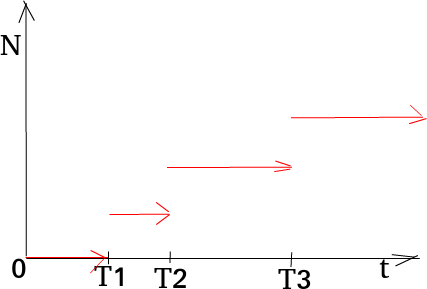
\includegraphics[width=.4\textwidth]{./pictures/3_17.png}
  \caption{График пуассоновского процесса}
  \label{fig:317}
\end{figure}

\subsubsection*{3.18}

\textit{Задание.}
Прибытие посетителей в магазин является процессом Пуассона с интенсивностью $ \lambda = 20$
посетителей в час.
Вычислите среднее количество продаж на протяжении одного восьмичасового рабочего дня,
если вероятность того, что посетитель магазина сделает покупку равна $0.3$.

\textit{Решение.}
$N \left( t \right) $ --- количество покупок за время $ \left[ 0, t \right] $.

Обозначим количество покупок как
$$n \left( t \right) =
  \sum \limits_{k = 1}^{N \left( t \right) } y_k,$$
где $y_k = \mathbbm{1}$\{$k$-й посетитель магазина сделает покупку\}.

При этом $P \left\{ y_k = 1 \right\} = 0.3$, а $P \left\{ y_k = 0 \right\} = 1 - 0.3 = 0.7$.

То есть $y_k$ имеет распределение Бернулли.

Из задачи 3.7 получает, что $n \left( t \right) \sim Pois \left( 0.3 \lambda \right) $.

Среднее количество покупок за 8 часов
$Mn \left( 8 \right) =
  8 \cdot 0.3 \lambda =
  8 \cdot 0.3 \cdot 20 =
  48$.

\subsubsection*{3.19}

\textit{Задание.}
Большой супермаркет имеет три входа.
Прибытие посетителей через каждые двери образуют процессы Пуассона с интенсивностями
$ \lambda_1 = 110, \, \lambda_2 = 90, \, \lambda_3 = 160$ посетителей в час.
30\% посетителей составляют мужчины.
Вероятность того, что посетитель-мужчина сделает покурку, равна $0.8$, а вероятность того,
что женщина-посетитель сделает покупку, равна $0.1$.
Средняя цена покупки составляет 100 грн.
\begin{enumerate}[label=\alph*)]
  \item Вычислите среднюю выручку супермаркета за 10-часовой рабочий день.
  \item Вычислите вероятность того, что третья женщина-посетитель, которая сделает покупку,
  прибудет в магазин в первые 15 минут.
  Вычислите среднее время её прибытия в магазин.
\end{enumerate}

\textit{Решение.}
\begin{enumerate}[label=\alph*)]
  \item $t = 10$.

  Найдём общую интенсивность $ \lambda = 110 + 90 + 160 = 360$ посетителей в час.

  Найдём $ \lambda_m = 360 \cdot 0.3 = 108$ посетителей-мужчин в час и
  $$ \lambda_w =
    360 \cdot 0.7 =
    252$$
  посетителей-женщин в час.

  Пусть $n \left( t \right) $ --- число покупок в день.
  Тогда
  $$Mn \left( t = 10 \right) =
    M \left[ n_m \left( 10 \right) + n_w \left( 10 \right) \right] =
    10 \cdot 108 \cdot 0.8 + 10 \cdot 252 \cdot 0.1 =
    1116.$$

  Следовательно, средняя выручка равна
  $$100Mn \left( t = 10 \right) =
    100 \cdot 1116 =
    111600.$$
  \item Пусть $ \lambda_w'$ --- интенсивность покупок, сделанных женщинами.

  $ \lambda_w' = \lambda_w \cdot 0.1 = 25.2$ покупки в час.

  Пусть $N \left( t \right) \sim Pois \left( \lambda_w' t \right) $ ---
  количество женщин-посетителей, прибывших в магазин до момента времени $t$.

  Тогда
  \begin{gather*}
    P \left\{ N \left( 15 minutes \right) = 3 \right\} =
    P \left\{ N \left( \frac{1}{4} \right) = 3 \right\} =
    e^{-25.2 \cdot \frac{1}{4}} \cdot \frac{ \left( -\frac{1}{4} \cdot 25.2 \right)^3}{3!} = \\
    = e^{-6.3} \cdot \frac{250}{6} =
    0.0019 \cdot 41.6 =
    0.08.
  \end{gather*}

  Тогда среднее время её прибытия в магазин
  $$M \tau =
    \frac{3}{ \lambda_w'} =
    \frac{3}{25.2} =
    0.12$$
  часов.
\end{enumerate}
